% ============================================================
% WHAT IS THIS FILE?
% This is a LaTeX file — it is the "source" of your document,
% just like HTML is the source of a webpage.
% You compile it (press the green Play/Build button in your
% LaTeX editor, e.g. TeXstudio or Overleaf) to produce the PDF.
%
% COMMENTS: Any line that starts with % is a comment.
%   Comments do NOT appear in the final PDF.
%   Use them to leave notes for yourself.
%
% HOW TO ADD A NEW LINE:
%   - Leave a BLANK LINE between text to start a new paragraph
%     (just like pressing Enter twice in Word).
%   - Use \\ at the end of a line to force a line break
%     (like Shift+Enter in Word — keeps you in the same paragraph).
%
% HOW TO ADD BOLD / ITALIC:
%   Bold:   \textbf{your text here}
%   Italic: \textit{your text here}
% ============================================================

\documentclass[11pt]{article}

% --- Font and encoding packages (leave these as-is) ---
\usepackage{times}
\usepackage{latexsym}
\usepackage[T1]{fontenc}
\usepackage[utf8]{inputenc}
\usepackage{microtype}

% --- Package for inserting images ---
\usepackage{graphicx}

% --- Package for clickable hyperlinks and references ---
\usepackage{hyperref}

% --- Package for citation styles (author, year) ---
\usepackage{natbib}

% ============================================================
% TITLE
% This is like the big heading at the top of your Word document.
% Replace the placeholder text between the { } with your title.
% ============================================================
\title{Optimizing Cross-Lingual Embeddings for isiZulu, Sepedi, 
and Setswana: Alignment Strategies, Pivot Selection, and 
Morphological Challenges \\[0.4em]
\medskip
\large Alignment Performance and Data Efficiency Across 
Conjunctive and Disjunctive Bantu Languages}
\bigskip

% ============================================================
% AUTHOR(S)
% This is your name and affiliation (e.g. university, department).
% Replace each placeholder with your details.
% If you have a SINGLE author, delete everything from \And onwards.
% If you have TWO authors, keep both blocks.
% ============================================================
\author{
  Tom Balay \\          
  Faculty of Engineering Built Environment and IT 
  University of Pretoria \\
  \texttt{u26853389@tuks.co.za}        
  % ---- DELETE the \and block below if you are the only author ----
  \and
  Franco van der Westhuizen  \\          
  Faculty of Engineering Built Environment and IT 
  University of Pretoria \\
  \texttt{u23543729@tuks.co.za}        
  \and
  Ndamulelo Mulaudzi \\
  Faculty of Engineering Built Environment and IT 
  University of Pretoria \\
  \texttt{u25715705@tuks.co.za} 
  \and
  Group 40       
}

% ============================================================
% DOCUMENT BEGINS HERE
% Everything between \begin{document} and \end{document}
% is the actual content of your report.
% ============================================================
\begin{document}
\maketitle   % This command prints the title, author and date at the top.

% ============================================================
% ABSTRACT
% A short summary of your whole report (usually 150-250 words).
% In Word this would just be a paragraph labelled "Abstract".
% ============================================================
\begin{abstract}
  Abstract paragraph goes here. Summarise your problem, your approach,
  your main results, and your conclusion in a few sentences.
\end{abstract}

% ============================================================
% SECTION — like "Heading 1" in Word
% Use \section{Heading name} to create a numbered section.
% LaTeX numbers them automatically (1, 2, 3 ...).
% ============================================================

\section{Introduction}
% ---- Write your introduction paragraphs below ----

South Africa currently gives constitutional recognition to eleven
official languages. This reflects a national commitment cultural
diversity and the accompanying linguistic equity. However, this
commitment is largely unrealized in digital technologies as 
evidenced by their underrepresentation in natural language processing 
(NLP) researh and infrastructure. The consequence is a widening 
accessibility gap where speakers of these languages are systematically 
excluded from the benefits of language technologies that speakers of 
high-resource languages such as English or French take for granted. 
Search engines, virtual assistants, machine translation systems, and 
automated information retrieval tools all presuppose the availability 
of large, well-annotated corpora — resources that remain scarce for 
the majority of South Africa's official languages.

Cross-lingual word embeddings offer a principled mechanism to address
this scarcity. The objective here is to transfer information from
high-resourced languages to low-resourced languages by projecting 
independently learned monolingual embeddings into a shared multilingual
represetation space. This way, a model trained on a high-resourced
language like English can generalize to lower resourced languages. This
transfer learning paradigm has demonstrated considerable promise across
different downstream NLP tasks such as named entity recognition (NER), 
part-of-speech tagging, and sentiment analysis. However, alignment quality 
is not language-agnostic — it is conditioned on the morphological structure 
of the target language. IsiZulu employs a conjunctive orthographic convention, 
fusing multiple morphemes into single written tokens, while Sepedi and Setswana 
follow a disjunctive convention, writing morphemes as discrete tokens. This 
distinction has direct implications for the geometry of the resulting embedding 
spaces and for the behaviour of alignment algorithms operating over them.

This study investigates whether CCA outperforms VecMap and KCCA across these 
morphologically distinct language pairs, and whether data volume requirements 
for effective alignment differ between conjunctive and disjunctive languages 
— with downstream named entity recognition (NER) as the evaluation task. These 
questions bear on a broader ethical imperative: language technology that functions 
only for a subset of a population's languages encodes structural inequality in software. 
South Africa's multilingual context makes it both an urgent case study and a 
generalisable test bed for low-resource NLP methodology, with findings intended to 
inform alignment method selection and data collection strategies across the African 
continent and beyond.
% ============================================================
% SUBSECTION — like "Heading 2" in Word
% Use \subsection{Heading name} inside a section.
% LaTeX numbers them automatically (1.1, 1.2 ...).
% ============================================================

\subsection{Problem Statement}
% ---- Write your problem statement below ----

Subsection paragraph goes here. Describe the specific problem you are solving.

\subsection{Objectives}
% ---- List your objectives below ----

Subsection paragraph goes here. State the goals of your project.

% ============================================================
% SUBSUBSECTION — like "Heading 3" in Word
% Use \subsubsection{Heading name} inside a subsection.
% ============================================================

% Example (uncomment the two lines below if you need a Heading 3):
% \subsubsection{Sub-subheading goes here}
% Paragraph goes here.

% ============================================================

\section{Related Work}

Section paragraph goes here. Review existing work relevant to your topic.

Second paragraph goes here. Discuss how your work differs or builds on prior work.

% ============================================================
% CITATION — like inserting a reference in Word
%
% Step 1: Add your reference to the file  custom.bib
%         (see the bottom of this file for how that works).
%
% Step 2: Cite it in your text using one of these commands:
%   \citet{key}   → Author (Year)      e.g.  Smith (2020) showed ...
%   \citep{key}   → (Author, Year)     e.g.  ... was shown \citep{Smith2020}.
%
% Replace "AuthorYear" below with the key from your .bib file.
% ============================================================

Citation example: as shown by \citet{AuthorYear}, paragraph continues here.
Another citation example: previous work supports this \citep{AnotherAuthorYear}.

% ============================================================

\section{Methodology}

\subsection{Subheading goes here}

Paragraph goes here. Describe your approach or method.

\subsection{Subheading goes here}

Paragraph goes here. Continue describing your methodology.

% ============================================================
% FIGURE — like inserting an image in Word
%
% Put your image file (e.g. my-diagram.png) in the SAME folder
% as this .tex file, then replace "my-diagram" below with
% the filename (without the extension).
%
% \caption{...}  is the caption that appears under the image.
% \label{...}    is a hidden tag so you can refer to the figure
%                in your text with \ref{fig:my-diagram}.
% ============================================================

\begin{figure}[h]
  \centering
  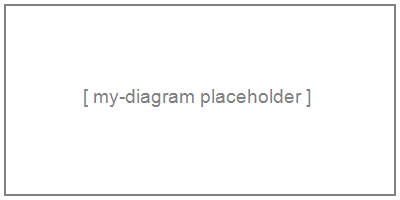
\includegraphics[width=\columnwidth]{my-diagram}   % <-- replace with your image filename
  \caption{Figure caption goes here.}
  \label{fig:my-diagram}
\end{figure}

% To refer to this figure in your text, write:
%   Figure~\ref{fig:my-diagram} shows ...

% ============================================================

\section{Results}

\subsection{Subheading goes here}

Paragraph goes here. Present your findings.

\subsection{Subheading goes here}

Paragraph goes here. Continue presenting results.

% ============================================================
% TABLE — like a table in Word
%
% {lcc} means three columns: left-aligned, centred, centred.
% Add or remove "c" or "l" or "r" columns as needed.
% Use & to move to the next column, and \\ to end a row.
% ============================================================

\begin{table}[h]
  \centering
  \begin{tabular}{lcc}
    \hline
    \textbf{Column Heading 1} & \textbf{Column Heading 2} & \textbf{Column Heading 3} \\
    \hline
    Row 1, Cell 1  & Row 1, Cell 2  & Row 1, Cell 3  \\
    Row 2, Cell 1  & Row 2, Cell 2  & Row 2, Cell 3  \\
    Row 3, Cell 1  & Row 3, Cell 2  & Row 3, Cell 3  \\
    \hline
  \end{tabular}
  \caption{Table caption goes here.}
  \label{tab:my-table}
\end{table}

% To refer to this table in your text, write:
%   Table~\ref{tab:my-table} shows ...

% ============================================================

\section{Discussion}

Paragraph goes here. Interpret your results and explain what they mean.

Second paragraph goes here. Discuss limitations of your work.

% ============================================================

\section{Conclusion}

Paragraph goes here. Summarise what you did and what you found.

Second paragraph goes here. Suggest directions for future work.

% ============================================================
% UNNUMBERED SECTIONS
% Adding * after \section makes it unnumbered (no number in front).
% Use this for Acknowledgements and Limitations — they are
% typically not numbered in academic reports.
% ============================================================

\section*{Limitations}

Paragraph goes here. Honestly describe the limitations of your work.

\section*{Acknowledgements}

Acknowledgements go here. Thank anyone who helped (supervisor, funding body, etc.).
% Example: This work was supervised by [Supervisor name goes here] at [Institution name goes here].

% ============================================================
% REFERENCES / BIBLIOGRAPHY
% This is automatically generated from your  custom.bib  file.
% Think of custom.bib as Word's "Manage Sources" list.
%
% To add a reference:
%   1. Open (or create)  custom.bib  in the same folder.
%   2. Add an entry like the example below.
%   3. Cite it in your text with \citet{} or \citep{}.
%
% Example .bib entry:
%
%   @article{Smith2020,
%     author  = {Smith, John},
%     title   = {Title of the Paper Goes Here},
%     journal = {Journal Name Goes Here},
%     year    = {2020},
%     volume  = {10},
%     pages   = {1--15},
%     doi     = {10.xxxx/xxxxx}
%   }
%
% The word before the comma on the first line ("Smith2020") is the
% KEY you use when you write \citet{Smith2020} in your text.
% ============================================================

\bibliographystyle{plainnat}   % citation style — leave this as-is
\bibliography{custom}          % points to your custom.bib file

% ============================================================
% APPENDIX (optional)
% Delete this whole section if you do not have an appendix.
% Appendix sections are labelled A, B, C ... automatically.
% ============================================================

\appendix

\section{Appendix Title Goes Here}
\label{sec:appendix-a}

Appendix paragraph goes here.

\end{document}
% ============================================================
% END OF DOCUMENT
% Nothing written below this line will appear in the PDF.
% ============================================================
